%%%%%%%%%%%%%%%%%%%%%%%%%%%%%%%%%%%%%%%%%%%%%%%%%%%%%%%%%%%%%%%%%%%%%%%%%%%%%%%
%% SOCIOL 723 -- Social Statistics II
%% Week 1 Thursday: OLS in Matrix Form
%% Wenhao Jiang, Duke University, Fall 2026
%%%%%%%%%%%%%%%%%%%%%%%%%%%%%%%%%%%%%%%%%%%%%%%%%%%%%%%%%%%%%%%%%%%%%%%%%%%%%%%

\documentclass[aspectratio=169,11pt,xcolor=dvipsnames]{beamer}
\mode<presentation>

%% ---- fonts: Latin Modern Roman (the LaTeX default), serif throughout -------
\usepackage[T1]{fontenc}
\usepackage{lmodern}
\usefonttheme{serif}
\renewcommand{\familydefault}{\rmdefault}

%% ---- packages --------------------------------------------------------------
\usepackage{amsmath,amsfonts,amssymb,bm}
\usepackage{graphicx}
\usepackage{booktabs}
\usepackage{tikz}
\usetikzlibrary{arrows.meta,positioning,calc}
\usepackage[english]{babel}

%% lightweight citation macros (beamer + natbib do not play well together)
\newcommand{\srcp}[1]{{\scriptsize\color{gray}(#1)}}   %% parenthetical
\newcommand{\srct}[1]{#1}                               %% inline / narrative

\DeclareMathOperator*{\argminop}{arg\,min}
\DeclareMathOperator*{\argmaxop}{arg\,max}
%% \limits forces the subscript underneath even in inline math
\newcommand{\argmin}{\argminop\limits}
\newcommand{\argmax}{\argmaxop\limits}
\DeclareMathOperator{\Cov}{Cov}
\DeclareMathOperator{\Var}{Var}
\DeclareMathOperator{\Corr}{Corr}
\DeclareMathOperator{\trace}{tr}
\DeclareMathOperator{\rank}{rank}
\DeclareMathOperator{\pcol}{col}
\newcommand{\indep}{\perp\!\!\!\perp}

%% ---- notation conventions (course-wide) ------------------------------------
%%  \E   population expectation (plain italic E)
%%  \En  sample / empirical expectation (blackboard-bold E)
%%  matrices and vectors are BOLD ITALIC via \bm, so they sit naturally
%%  alongside the italic scalar notation
\newcommand{\E}{E}
\newcommand{\En}{\mathbb{E}_n}
\newcommand{\R}{\mathbb{R}}
\newcommand{\X}{\bm{X}}
\newcommand{\Y}{\bm{y}}
\newcommand{\Ix}{\bm{I}}
\newcommand{\zero}{\bm{0}}
\newcommand{\one}{\bm{1}}
\newcommand{\Pm}{\bm{P}}
\newcommand{\Mm}{\bm{M}}
\newcommand{\bhat}{\hat{\bm{\beta}}}
\newcommand{\ehat}{\hat{\bm{e}}}

%% ---- theme -----------------------------------------------------------------
\usetheme{default}
%% thin single-line header: clickable section names, current one highlighted.
%% (miniframes is deliberately not used: one dot per slide wraps to 4 rows here)
\setbeamerfont{section in head/foot}{size=\tiny}
\setbeamertemplate{headline}{%
  \begin{beamercolorbox}[wd=\paperwidth,ht=2.4ex,dp=1.1ex,%
                         leftskip=.3cm,rightskip=.3cm]{section in head/foot}%
    \usebeamerfont{section in head/foot}%
    \insertsectionnavigationhorizontal{.94\paperwidth}{}{}%
  \end{beamercolorbox}%
}

\definecolor{dukeblue}{RGB}{1,33,105}
\definecolor{accent}{RGB}{200,78,0}
\definecolor{softgray}{RGB}{242,242,245}

\setbeamercolor{structure}{fg=dukeblue}
\setbeamercolor{frametitle}{fg=dukeblue,bg=white}
\setbeamercolor{section in head/foot}{fg=white,bg=dukeblue}
\setbeamercolor{section in head/foot shaded}{fg=white!50!dukeblue,bg=dukeblue}
\setbeamercolor{alerted text}{fg=accent}
\setbeamercolor{block title}{fg=white,bg=dukeblue}
\setbeamercolor{block body}{fg=black,bg=softgray}
\setbeamercolor{block title alerted}{fg=white,bg=accent}
\setbeamercolor{block body alerted}{fg=black,bg=softgray}

\setbeamertemplate{footline}[page number]
\setbeamertemplate{navigation symbols}{}
%% continued frames keep the SAME font size and spill onto a new slide
\setbeamertemplate{frametitle continuation}{\ifnum\insertcontinuationcount>1\normalfont\footnotesize\ (cont.)\fi}
\setbeamertemplate{itemize items}[circle]
\setbeamertemplate{blocks}[rounded][shadow=false]
\setbeamerfont{frametitle}{series=\bfseries}
\setbeamerfont{footnote}{size=\scriptsize}
\setbeamerfont{caption}{size=\footnotesize}
\setbeamertemplate{subsection in head/foot}{}
\setbeamertemplate{subsection in head/foot shaded}{}
\setbeamertemplate{caption}[numbered]

%% marker for material that is for understanding, not for examination
\newcommand{\adv}{\,\raisebox{0.6pt}{\textcolor{accent}{$\bigstar$}}}
%% marker for essential material every student must understand (examinable core)
\definecolor{corestar}{RGB}{0,83,155}
\newcommand{\core}{\,\raisebox{0.6pt}{\textcolor{corestar}{$\bigstar$}}}

%% section / subsection dividers
\setbeamertemplate{section page}{%
  \begin{centering}\vfill
  {\usebeamercolor[fg]{structure}\Large\bfseries\insertsectionhead\par}
  \vskip4pt{\color{dukeblue}\rule{0.35\linewidth}{1pt}\par}
  \vfill\end{centering}}
\setbeamertemplate{subsection page}{%
  \begin{centering}\vfill
  {\usebeamercolor[fg]{structure}\large\bfseries\insertsubsectionhead\par}
  \vfill\end{centering}}


%% tighter vertical rhythm: math-heavy beamer frames otherwise overflow
\AtBeginDocument{%
  \setlength{\abovedisplayskip}{5pt}%
  \setlength{\belowdisplayskip}{5pt}%
  \setlength{\abovedisplayshortskip}{2pt}%
  \setlength{\belowdisplayshortskip}{3pt}%
}
\setbeamertemplate{frametitle}{%
  \vskip4pt\usebeamerfont{frametitle}\usebeamercolor[fg]{frametitle}%
  \insertframetitle\par\vskip2pt}
\setbeamersize{text margin left=0.75cm, text margin right=0.75cm}

%% ---- title -----------------------------------------------------------------
%% ---- title page: same face as the body (Latin Modern), larger and bold
\setbeamerfont{title}{size*={16}{19},series=\bfseries}
\setbeamerfont{subtitle}{size=\Large,series=\mdseries}
\setbeamerfont{author}{size=\large}
\setbeamerfont{date}{size=\large}
\title[SOCIOL 723]{SOCIOL 723: Social Statistics II\\[4pt]}
\subtitle{Week 1 (Thursday), OLS in Matrix Form\\[-6pt]}
\author[Jiang]{Wenhao Jiang\vspace{-1.5em}}
\institute[Duke]{}
\titlegraphic{
\includegraphics[height=1.3cm]{../Misc/duke_logo.png}}
\date{Department of Sociology, Fall 2026}

\begin{document}

\begin{frame}[plain]
  \titlepage
\end{frame}

\begin{frame}{Today}
  \tableofcontents
  \vskip6pt
  {\footnotesize Tuesday built everything in scalar form. Today: the same
  objects again in matrix form, for general understanding, followed by lab.\\
  \core{} $=$ essential, you must understand this \quad\quad \adv{} $=$ for
  understanding, not examined}
\end{frame}

%%%%%%%%%%%%%%%%%%%%%%%%%%%%%%%%%%%%%%%%%%%%%%%%%%%%%%%%%%%%%%%%%%%%%%%%%%%%%%%
\section[Matrix Form]{The Matrix Form and Its Geometry}
%%%%%%%%%%%%%%%%%%%%%%%%%%%%%%%%%%%%%%%%%%%%%%%%%%%%%%%%%%%%%%%%%%%%%%%%%%%%%%%
\begin{frame}\sectionpage\end{frame}

\begin{frame}{Why Bother}
\begin{itemize}\itemsep5pt
  \item With $k$ regressors, scalar algebra needs $k$ normal equations and becomes
        unreadable. Matrix algebra stays two lines long for any $k$.
  \item The \alert{geometry}, projection onto a subspace, is invisible in
        scalar form and obvious in matrix form.
  \item In the literature, most estimators you will meet (fixed effects, IV,
        2SLS, ridge) are \emph{written} as small variations on
        $\bhat = (\X'\X)^{-1}\X'\Y$. We will keep working in scalars, but
        recognizing this form is what lets you read modern papers.
\end{itemize}
\vskip6pt
\begin{alertblock}{But}
Nothing in this section is new content. It is the \emph{same} normal equations
you derived on Tuesday, written more compactly. And the lab stays entirely in
scalar form: sums, means, and \texttt{lm()}, on simulations and the GSS.
\end{alertblock}
\end{frame}

\begin{frame}{Vectors and Matrices, From Zero\core}
No linear algebra is assumed in this course. Here is the part we need, from
nothing.
\begin{itemize}\itemsep3pt
  \item A \textbf{vector} is a list of numbers written in a column. $X_i$ is the
        list describing unit $i$: one entry per variable, with a $1$ on top for
        the intercept.
  \item A \textbf{matrix} is a rectangular table of numbers: an $n\times k$
        matrix has $n$ rows and $k$ columns.
  \item The \textbf{transpose} $'$ tips a column onto its side: if $X_i$ is a
        $k\times 1$ column, then $X_i'$ is the same list lying down, $1\times k$.
\end{itemize}
\vskip2pt
\begin{block}{The one formula to internalize}
\begin{align*}
  X_i'\bm\beta = \beta_0\cdot 1 + \beta_1 X_{i1} + \cdots + \beta_{k-1}X_{i,k-1} :
\end{align*}
a row times a column is a \emph{single number}: multiply matching entries, then
add. So $X_i'\bm\beta$ is nothing but unit $i$'s fitted value, written
compactly. Whenever you see $X_i'\bm\beta$, read it as ``the regression line
evaluated at unit $i$.''
\end{block}
\end{frame}

\begin{frame}{Multiplying and Inverting}
The only two operations we use. \textbf{Multiplication} extends the
row-times-column rule: entry $(r,c)$ of $\bm{AB}$ is (row $r$ of $\bm A$)
times (column $c$ of $\bm B$):
\begin{align*}
  \begin{bmatrix} 1 & 2 \\ 3 & 4 \end{bmatrix}
  \begin{bmatrix} 5 \\ 6 \end{bmatrix}
  =
  \begin{bmatrix} 1\cdot 5 + 2\cdot 6 \\ 3\cdot 5 + 4\cdot 6\end{bmatrix}
  = \begin{bmatrix} 17 \\ 39 \end{bmatrix}.
\end{align*}
Dimensions must match, $(n\times k)(k\times 1) = (n\times 1)$, and order
matters: $\bm{AB}\neq\bm{BA}$ in general.
\vskip2pt
\textbf{Inversion} is the matrix version of dividing. For a number,
$a^{-1}a = 1$; for a square matrix, $\bm A^{-1}\bm A = \Ix$, the
\emph{identity} matrix (ones on the diagonal, zeros elsewhere), which leaves
whatever it multiplies unchanged.
\begin{itemize}\itemsep2pt
  \item Just as $1/a$ fails to exist when $a = 0$, $\bm A^{-1}$ fails to exist
        when the matrix collapses information; that is the ``rank'' condition,
        explained shortly.
  \item You will never invert a matrix by hand here; \texttt{R}'s
        \texttt{solve()} does it. What matters is knowing what the symbol says.
\end{itemize}
\end{frame}

\begin{frame}{Stacking the Data}
For $n$ units and $k$ regressors (including the constant):
\begin{align*}
  \Y = \begin{bmatrix} Y_1 \\ \vdots \\ Y_n \end{bmatrix}_{n\times 1},
  \quad
  \X = \begin{bmatrix} X_1' \\ \vdots \\ X_n' \end{bmatrix}
     = \begin{bmatrix}
        1 & X_{11} & \cdots & X_{1,k-1}\\
        \vdots & \vdots & & \vdots \\
        1 & X_{n1} & \cdots & X_{n,k-1}
       \end{bmatrix}_{n\times k},
  \quad
  \bm\epsilon = \begin{bmatrix} \epsilon_1 \\ \vdots \\ \epsilon_n\end{bmatrix}.
\end{align*}
The model, stacked over units:
\begin{align*}
  \Y = \X\bm\beta + \bm\epsilon
  \qquad\Longleftrightarrow\qquad
  Y_i = X_i'\bm\beta + \epsilon_i,\quad i=1,\dots,n .
\end{align*}
Two objects do all the work:
$\ \X'\X = \sum_i X_iX_i'$ (a $k\times k$ matrix) and
$\ \X'\Y = \sum_i X_i Y_i$ (a $k\times 1$ vector).
\end{frame}

\begin{frame}{Least Squares in Matrix Form: the Expansion}
The sum of squared errors is the error vector times itself:
\begin{align*}
  S(b) = \sum_{i} (Y_i - X_i'b)^2 = (\Y-\X b)'(\Y-\X b) .
\end{align*}
\begin{block}{Two transpose rules, used constantly}
$(\bm A + \bm B)' = \bm A' + \bm B'$, and $(\bm A\bm B)' = \bm B'\bm A'$:
transposing a product \emph{reverses the order}. Hence $(\X b)' = b'\X'$.
\end{block}
Multiply out, term by term:
\begin{align*}
  S(b) = \Y'\Y - \Y'\X b - b'\X'\Y + b'\X'\X b
       = \Y'\Y - 2\,b'\X'\Y + b'\X'\X b .
\end{align*}
\vskip-2pt
\begin{itemize}\itemsep2pt
  \item Why do the middle terms merge? Each is $1\times1$, a single number,
        and a number equals its own transpose: $(b'\X'\Y)' = \Y'\X b$. The two
        terms are the \emph{same} number written twice.
\end{itemize}
\end{frame}

\begin{frame}{Minimizing: Two Matrix Derivatives, From Zero}
$\partial S/\partial b$ just stacks the $k$ partials into a column; two
stock rules cover everything:
\begin{block}{The rules, with their scalar shadows}
\begin{align*}
  \frac{\partial (a'b)}{\partial b} &= a
  &&\text{since } a'b = \textstyle\sum_j a_jb_j
    \text{ gives } \partial/\partial b_j = a_j
  &&\text{(cf.\ } \tfrac{d}{db}\,ab = a\text{)} \\[2pt]
  \frac{\partial (b'\bm Ab)}{\partial b} &= 2\bm Ab
  &&\text{for symmetric } \bm A
  &&\text{(cf.\ } \tfrac{d}{db}\,ab^2 = 2ab\text{)}
\end{align*}
\end{block}
Apply them with $a = \X'\Y$ and $\bm A = \X'\X$ (symmetric):
\begin{align*}
  \frac{\partial S(b)}{\partial b} = -2\X'\Y + 2\X'\X b \overset{!}{=} 0
  \quad\Longrightarrow\quad
  \underbrace{\X'\X\,\bhat = \X'\Y}_{\text{\alert{normal equations}}} .
\end{align*}
\vskip-2pt
The \emph{same} $k$ equations you wrote out one at a time on Tuesday.
{\footnotesize Why a minimum? $v'\X'\X v = \|\X v\|^2 \geq 0$ for all $v$:
$S$ is a bowl. (Shorthand: $\X'\X \succeq 0$, the matrix $\geq$.)}
\end{frame}

\begin{frame}{The Normal Equations, Slowly: the Bivariate Case}
Take $k=2$ with $X_i = (1, X_i)'$, so $b = (b_0, b_1)'$. The two building
blocks are
\begin{align*}
  \X'\X = \begin{bmatrix} n & \sum_i X_i \\ \sum_i X_i & \sum_i X_i^2 \end{bmatrix},
  \qquad
  \X'\Y = \begin{bmatrix} \sum_i Y_i \\ \sum_i X_iY_i \end{bmatrix} .
\end{align*}
Write out $\X'\X\bhat = \X'\Y$ one row at a time:
\begin{align*}
  n\hat\beta_0 + \hat\beta_1\textstyle\sum_i X_i = \textstyle\sum_i Y_i
  \;&\Longleftrightarrow\;
  \textstyle\sum_i\big(Y_i - \hat\beta_0 - \hat\beta_1X_i\big) = 0 \\[2pt]
  \hat\beta_0\textstyle\sum_i X_i + \hat\beta_1\textstyle\sum_i X_i^2
  = \textstyle\sum_i X_iY_i
  \;&\Longleftrightarrow\;
  \textstyle\sum_i X_i\big(Y_i - \hat\beta_0 - \hat\beta_1X_i\big) = 0
\end{align*}
\vskip2pt
\begin{itemize}\itemsep2pt
  \item Row by row, the matrix equation \emph{is} Tuesday's (N1) and (N2):
        residuals sum to zero, and residuals are orthogonal to the regressor.
  \item One matrix line, $k$ scalar equations. That is the entire content of
        the compact notation: nothing new, everything stacked.
\end{itemize}
\end{frame}


\begin{frame}{The Estimator, Existence, and Rank}
\begin{block}{What ``rank'' means, in words}
The \alert{rank} of $\X$ is the number of genuinely distinct columns it
contains: columns that cannot be rebuilt as combinations of the others.
\emph{Full column rank}, $\rank(\X)=k$, says no column is redundant: the data
carry $k$ separate pieces of information, one per coefficient.
\end{block}
\begin{block}{The OLS estimator}
If $\rank(\X)=k$, $\X'\X$ is invertible and
\begin{align*}
  \bhat = (\X'\X)^{-1}\X'\Y = \big(\En[X_iX_i']\big)^{-1}\En[X_iY_i] .
\end{align*}
\end{block}
\begin{itemize}\itemsep2pt
  \item Full rank needs $n \geq k$; it is the matrix version of ``$X$ must
        vary.''
  \item Failures you will actually meet: the \emph{dummy variable trap}; including
        a variable and a rescaling of it; a group indicator constant within a
        fixed effect.
  \item If rank fails, \texttt{R} silently drops a column and reports \texttt{NA}.
        That \texttt{NA} is never a mystery.
\end{itemize}
\end{frame}

\begin{frame}{Sanity Check: Recovering the Scalar Formula\adv}
Let $k=2$ with $X_i = (1, X_i)'$. Then
\begin{align*}
  \X'\X = \begin{bmatrix} n & \sum_i X_i \\ \sum_i X_i & \sum_i X_i^2\end{bmatrix},
  \qquad
  \X'\Y = \begin{bmatrix} \sum_i Y_i \\ \sum_i X_i Y_i \end{bmatrix} .
\end{align*}
Using $\begin{bmatrix} a & b\\ c& d\end{bmatrix}^{-1}
= \frac{1}{ad-bc}\begin{bmatrix} d & -b\\ -c & a\end{bmatrix}$,
\begin{align*}
  \hat\beta_1 = \frac{n\sum_i X_iY_i - \sum_i X_i \sum_i Y_i}
                     {n\sum_i X_i^2 - (\sum_i X_i)^2}
  = \frac{\Cov_n(X,Y)}{\Var_n(X)},
  \qquad
  \hat\beta_0 = \bar Y - \hat\beta_1 \bar X .
\end{align*}
\vskip4pt
Exactly what we derived by hand. The matrix form is a change of language, not of
substance.
\end{frame}

\begin{frame}{Why Projection? It Is Tuesday's Argmin, Re-Read\adv}
Tuesday defined OLS by a minimization:
$\ \bhat = \argmin_b \sum_{i=1}^n (Y_i - X_i'b)^2$.
\begin{block}{The one observation everything hangs on}
A sum of squared entries is a squared \emph{length}:
$\ \sum_{i} (Y_i - X_i'b)^2 = \|\Y - \X b\|^2$, the squared \emph{distance}
between two points of $\R^n$, the data $\Y$ and the candidate fit $\X b$. So
the argmin says, word for word: \alert{among all fits the model can produce,
pick the one closest to the data.}
\end{block}
\begin{itemize}\itemsep2pt
  \item The candidate fits $\X b$ form a flat sheet, a ``plane'' (next
        frame), and ``closest point on a plane'' is a problem geometry solved
        long before calculus: \alert{the foot of the perpendicular}.
  \item The right angle \emph{is} the first-order condition: perpendicular to
        every column of $\X$ means $\X'\ehat = \zero$, the normal equations,
        with no differentiation anywhere.
  \item Nothing new is computed: projection is the same argmin,
        \emph{answered by geometry instead of calculus}. Next: the smallest
        possible case.
\end{itemize}
\end{frame}

\begin{frame}{What Does ``All the Fits'' Look Like?\adv}
Read matrix-times-vector as a \alert{recipe for mixing columns}:
\begin{align*}
  \X b = b_1\cdot(\text{column }1) + b_2\cdot(\text{column }2)
       + \cdots + b_k\cdot(\text{column }k) :
\end{align*}
each coefficient pours in that much of its column. The set of candidate fits
is therefore \emph{every possible mixture of the $k$ columns}.
\begin{itemize}\itemsep1pt
  \item \textbf{One column} (intercept only): the mixtures are all multiples
        of $\one$, a \alert{line} through the origin. Projecting $\Y$ onto
        that line gives $\hat b = \bar Y$: \alert{the sample mean is a
        projection}.
  \item \textbf{Two columns}: the mixtures of two arrows fill a flat
        \alert{plane} through the origin.
  \item \textbf{$k$ columns}: the mixtures fill a $k$-dimensional flat
        subspace of $\R^n$. ``$k$-dimensional'' simply counts the free
        coefficients $b_1,\dots,b_k$.
  \item $\Y$ generally sits \emph{off} this subspace; the gap is the
        residual. A column that is itself a mixture of the others adds no new
        direction, so the subspace has dimension below $k$: \alert{rank},
        again.
\end{itemize}
\end{frame}

\begin{frame}{The Picture: $n = 3$, Two Columns\adv}
Three observations ($n=3$), two columns: $\X = [\,\one \ \ \bm x\,]$ is
$3\times2$.
The mixtures $b_0\one + b_1\bm x$ fill the shaded plane; the data $\Y$ floats
\emph{off} it, in the third dimension.
\begin{center}
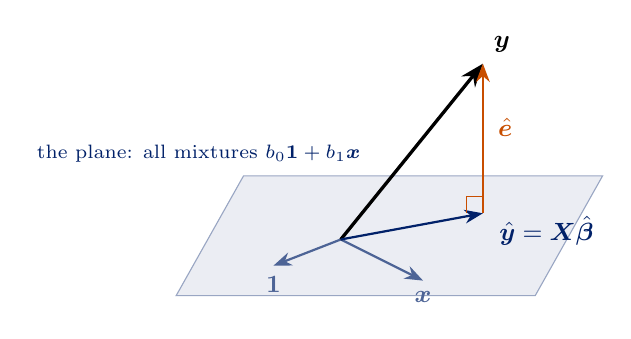
\begin{tikzpicture}[scale=0.95,>=Stealth]
  \fill[dukeblue!8] (-2.2,-0.75) -- (2.6,-0.75) -- (3.5,0.85) -- (-1.3,0.85) -- cycle;
  \draw[dukeblue!40] (-2.2,-0.75) -- (2.6,-0.75) -- (3.5,0.85) -- (-1.3,0.85) -- cycle;
  \node[dukeblue] at (-1.9,1.15) {\scriptsize the plane: all mixtures $b_0\one + b_1\bm{x}$};
  \coordinate (O) at (0,0);
  \coordinate (Yhat) at (1.9,0.35);
  \coordinate (Y) at (1.9,2.35);
  \draw[->,dukeblue!70,thick] (O) -- (-0.9,-0.35) node[below] {\small $\one$};
  \draw[->,dukeblue!70,thick] (O) -- (1.1,-0.55) node[below] {\small $\bm x$};
  \draw[->,very thick] (O) -- (Y) node[above right] {\small $\Y$};
  \draw[->,thick,dukeblue] (O) -- (Yhat);
  \node[dukeblue] at (2.75,0.12) {\small $\hat\Y = \X\bhat$};
  \draw[->,thick,accent] (Yhat) -- (Y);
  \node[accent] at (2.2,1.5) {\small $\ehat$};
  \draw[accent] ($(Yhat)+(0,0.22)$) -- ($(Yhat)+(-0.22,0.22)$) -- ($(Yhat)+(-0.22,0)$);
\end{tikzpicture}
\end{center}
\vskip-4pt
\begin{itemize}\itemsep2pt
  \item OLS drops the perpendicular from $\Y$ to the plane: the foot is the
        fit $\hat\Y$, the gap is the residual $\ehat$. Perpendicular to the
        plane $=$ perpendicular to \emph{both} columns: $\X'\ehat = \zero$,
        the normal equations.
  \item Fitting is dropping a perpendicular. Everything else is bookkeeping.
\end{itemize}
\end{frame}


\begin{frame}{Deriving $\bhat$ from the Picture, No Calculus\adv}
The picture makes its own demand: the residual must be \alert{perpendicular
to the plane}, that is, perpendicular to \emph{every column} of $\X$. Written
in one matrix line, and then rearranged:
\begin{align*}
  \X'\big(\Y - \X\bhat\big) = \zero
  \quad\Longrightarrow\quad
  \X'\X\,\bhat = \X'\Y
  \quad\Longrightarrow\quad
  \bhat = (\X'\X)^{-1}\X'\Y .
\end{align*}
\begin{itemize}\itemsep3pt
  \item The first equality \emph{is} the perpendicularity requirement; the
        rest is rearranging. \alert{Same normal equations, same estimator,
        and not a derivative in sight.} Geometry and calculus are two proofs
        of one formula.
  \item Substituting back, the fitted vector is
        $\hat\Y = \X\bhat = \X(\X'\X)^{-1}\X'\,\Y$: one matrix carries the
        data straight to the fit.
\end{itemize}
\vskip2pt
{\footnotesize Names you will meet in the literature: $\Pm = \X(\X'\X)^{-1}\X'$
is the \emph{hat matrix} (it puts the hat on $\Y$), and $\Mm = \Ix_n - \Pm$
the \emph{residual maker} ($\ehat = \Mm\Y$). We will not need their algebra.}
\end{frame}









%%%%%%%%%%%%%%%%%%%%%%%%%%%%%%%%%%%%%%%%%%%%%%%%%%%%%%%%%%%%%%%%%%%%%%%%%%%%%%%
\section[Partialling Out]{Partialling Out in General}
%%%%%%%%%%%%%%%%%%%%%%%%%%%%%%%%%%%%%%%%%%%%%%%%%%%%%%%%%%%%%%%%%%%%%%%%%%%%%%%
\begin{frame}\sectionpage\end{frame}

\begin{frame}{The Frisch--Waugh--Lovell Theorem\adv}
Partition $\X = [\,\X_1\ \ \X_2\,]$: a treatment of interest and controls.
Let $\Mm_2 = \Ix - \X_2(\X_2'\X_2)^{-1}\X_2'$ and define
\begin{align*}
  \tilde{\X}_1 = \Mm_2\X_1 ,
  \qquad
  \tilde{\Y} = \Mm_2\Y .
\end{align*}
\begin{block}{Theorem}
The OLS estimate $\hat{\bm\beta}_1$ from the full regression equals
\begin{align*}
  \hat{\bm\beta}_1
  = (\tilde\X_1'\tilde\X_1)^{-1}\tilde\X_1'\,\tilde\Y
  \;=\; (\tilde\X_1'\tilde\X_1)^{-1}\tilde\X_1'\,\Y
  \qquad (\text{note: } \tilde\Y \text{ vs.\ raw } \Y) ,
\end{align*}
\end{block}
\vskip1pt
The two right-hand sides differ only in the tilde on $\Y$; they are equal for
Tuesday's reason (the part removed from $\Y$ is built from $\X_2$, to which
$\tilde\X_1$ is orthogonal). Tuesday's three-step recipe, any number of controls.
\end{frame}

\begin{frame}{Proof of FWL\adv}
Start from the \emph{fitted} full regression, an exact identity in the sample:
\begin{align*}
  \Y = \X_1\hat{\bm\beta}_1 + \X_2\hat{\bm\beta}_2 + \ehat .
\end{align*}
Premultiply once by $\Mm_2$, using $\Mm_2\X_2 = \zero$ and
$\Mm_2\ehat = \ehat$ ($\ehat$ already has $\X_2$ removed, since
$\X_2'\ehat = \zero$):
\begin{align*}
  \tilde\Y = \tilde\X_1\hat{\bm\beta}_1 + \ehat .
\end{align*}
Now regress $\tilde\Y$ on $\tilde\X_1$:
\begin{align*}
  (\tilde\X_1'\tilde\X_1)^{-1}\tilde\X_1'\tilde\Y
  = \hat{\bm\beta}_1
  + (\tilde\X_1'\tilde\X_1)^{-1}\underbrace{\tilde\X_1'\ehat}_{=\,\zero}
  = \hat{\bm\beta}_1 ,
\end{align*}
because $\tilde\X_1'\ehat = \X_1'\Mm_2\ehat = \X_1'\ehat = \zero$ (using
$\Mm_2' = \Mm_2$, visible by transposing its definition). $\blacksquare$
\end{frame}

\begin{frame}{Why FWL Matters More Than It Looks}
\begin{enumerate}\itemsep6pt
  \item \textbf{Interpretation.} ``Controlling for $W$'' $=$ discarding all
        covariance between $X_1$ and $W$. Your estimate lives on what remains.
  \item \textbf{Diagnostics.} The added-variable plot is the only two-dimensional
        picture that faithfully represents a multivariate slope.
  \item \textbf{Generality.} Nothing in the argument requires $\X_2$ to enter
        linearly, it only requires that we can compute the part of $X_1$ that
        $\X_2$ predicts. That observation is the seed of a large literature, and
        we return to it briefly in Week 13.
\end{enumerate}
\end{frame}

\begin{frame}{Where This Leaves Us}
\begin{itemize}\itemsep5pt
  \item OLS minimizes squared errors. Everything else, the slope formula, the
        normal equations, FWL, OVB, follows from that one criterion by algebra.
  \item In the population, OLS estimates the best linear approximation to the CEF.
        Under A1--A4 the sample version is unbiased for it.
  \item Whether that coefficient is a \emph{causal effect} is a separate question
        that regression cannot answer.
  \item \textbf{Next week}: we have $\hat\beta$; now we need to know how uncertain
        it is, and the standard error your software prints is usually the wrong
        one.
\end{itemize}
\vskip6pt
\begin{block}{This week's reading}
MHE Chapter 3; CCI Chapter 6. The lab computes OLS by hand in scalar form,
on simulated data and the GSS; no matrix computations anywhere.
\end{block}
\end{frame}

\begin{frame}[allowframebreaks,t]{References}
\footnotesize
\begin{itemize}\itemsep3pt
\item Angrist, Joshua D. and J\"orn-Steffen Pischke. 2009.
\textit{Mostly Harmless Econometrics}. Princeton University Press. [Ch.\ 3]
\item Morgan, Stephen L. and Christopher Winship. 2015.
\textit{Counterfactuals and Causal Inference}, 2nd ed. Cambridge University Press.
[Ch.\ 6]
\item James, Gareth, Daniela Witten, Trevor Hastie, and Robert Tibshirani. 2021.
\textit{An Introduction to Statistical Learning}, 2nd ed. Springer. [Ch.\ 2--3]
\item Arbatl{\i}, Cemal Eren, Quamrul H. Ashraf, Oded Galor, and Marc Klemp.
2020. ``Diversity and Conflict.'' \textit{Econometrica} 88(2): 727--797.
[the added-variable plot example]
\item Correll, Josh, Abigail M. Folberg, Charles M. Judd, Gary H. McClelland, and
Carey S. Ryan. 2024. \textit{Data Analysis: A Model Comparison Approach to
Regression, ANOVA, and Beyond}, 4th ed. Routledge. [for review]
\end{itemize}
\end{frame}

\end{document}
